%%
%% Post-Quantum Laconic Private Set Intersection:
%% First Empirical Implementation and Performance Evaluation
%% Information Sciences — Elsevier — Submission Draft
%%
\documentclass[preprint,12pt]{elsarticle}

%% ── Packages ─────────────────────────────────────────────────────────────────
\usepackage{amsmath,amssymb,amsthm}
\usepackage{booktabs}
\usepackage{graphicx}
\usepackage{algorithm}
\usepackage{algorithmic}
\usepackage{multirow}
\usepackage{tabularx}
\usepackage{enumitem}
\usepackage{lineno}
\usepackage{microtype}
\usepackage{hyperref}
\usepackage{xcolor}
\usepackage[capitalize,nameinlink]{cleveref}

%% ── Journal ──────────────────────────────────────────────────────────────────
\journal{Information Sciences}

%% ── Theorem environments ─────────────────────────────────────────────────────
\newtheorem{theorem}{Theorem}
\newtheorem{proposition}[theorem]{Proposition}
\newtheorem{lemma}[theorem]{Lemma}
\newtheorem{definition}{Definition}
\newtheorem{remark}{Remark}

%% ── Crypto shorthand ─────────────────────────────────────────────────────────
\newcommand{\DKLLMR}{\textsc{DKLLMR23}}
\newcommand{\laconicenc}{\textsf{LaconicEnc}}
\newcommand{\laconicdec}{\textsf{LaconicDec}}
\newcommand{\keygen}{\textsf{KeyGen}}
\newcommand{\upd}{\textsf{Upd}}
\newcommand{\witgen}{\textsf{WitGen}}
\newcommand{\Rq}{R_q}
\newcommand{\Zq}{\mathbb{Z}_q}

%% ── Distributed footnote marker ──────────────────────────────────────────────
%% All projected distributed figures use this unified marker.
\newcommand{\projdagger}{${}^\dagger$}

% =============================================================================
\begin{document}
\begin{frontmatter}

%% ── Title ────────────────────────────────────────────────────────────────────
\title{Laconic Private Set Intersection from Ring-LWE:\\ Implementation and Performance Evaluation}

%% ── Authors ──────────────────────────────────────────────────────────────────
\author[iiitk]{Ceemala Venkata Santhosh Kumar Reddy\corref{cor1}}
\ead{santhoshcheemala6303@gmail.com}
\cortext[cor1]{Corresponding author}

\author[iiitk]{A. Balu}
\ead{balu@iiitkottayam.ac.in}

\affiliation[iiitk]{
  organization={Department of Cyber Security, Indian Institute of Information
                Technology Kottayam},
  city={Kottayam},
  state={Kerala},
  postcode={686635},
  country={India}
}

%% ── Abstract ─────────────────────────────────────────────────────────────────
\begin{abstract}
Private Set Intersection (PSI) enables two mutually distrusting parties to
compute the overlap of their datasets without revealing any non-matching
elements. Existing high-performance PSI protocols rely on discrete-logarithm
or oblivious-transfer (OT) based assumptions---both of which are broken by
Shor's algorithm on a sufficiently large quantum computer---making them
unsuitable for long-lived sensitive data subject to ``harvest now, decrypt
later'' (HNDL) attacks.

Laconic PSI achieves sublinear $O(n \log m)$ communication and produces a
reusable server digest, yet post-quantum constructions have until now lacked
any implementation or empirical evidence of feasibility. We close this gap by
presenting the first end-to-end implementation and empirical evaluation of a
Ring-LWE-based laconic PSI protocol in Go, under standard semi-honest security
(both parties learn the intersection and nothing more).

Our key findings are threefold. First, server initialisation (${\approx}29\%$)
and per-record intersection (${\approx}69\%$) dominate wall-clock time; Lattigo
NTT ring operations account for $\approx 28\%$ of CPU samples (measured via
\texttt{pprof} at $M=100$, $D=256$), identifying GPU-NTT acceleration as the
highest-value optimisation target. Second, a sharded distributed deployment
across $K$ nodes reduces per-node work linearly: $K=8$ nodes are projected to
reduce latency from the single-node baseline of 163.1 minutes to under
25~minutes\projdagger. Third, NIST PQC Level~1 parameters ($D=2048$) impose a
$3.2$--$21.6\times$ overhead over 64-bit parameters, establishing the first
concrete cost model for lattice-strengthening in laconic PSI.

We additionally introduce \textbf{FLARE}, a proof-of-concept
sanctions-screening application demonstrating that post-quantum,
privacy-preserving compliance is feasible on commodity infrastructure.

\smallskip\noindent
\textit{Note on projected figures:} All distributed timing estimates
(marked \projdagger) are linear-scaling projections from single-node
measurements; GCE cluster benchmarks are pending.
\end{abstract}

%% ── Keywords ─────────────────────────────────────────────────────────────────
\begin{keyword}
Private Set Intersection \sep Laconic Cryptography \sep Ring-LWE \sep
Post-Quantum Cryptography \sep Privacy-Preserving Computation \sep
Sanctions Screening \sep Distributed Systems
\end{keyword}

\end{frontmatter}

\linenumbers   % enable for review submission

% =============================================================================
\section{Introduction}
\label{sec:intro}
% =============================================================================

A European bank must screen thousands of customers daily against
government-mandated sanctions lists---yet sharing those customer identifiers
with an external screening provider violates GDPR's data-minimisation
principle. Anti-money laundering law demands screening; privacy law prohibits
disclosure. This is not a niche edge case; it is a structural conflict faced
by every regulated financial institution on the continent.

\emph{Private Set Intersection} (PSI) resolves this dilemma: two parties
compute the intersection of their datasets without revealing any non-matching
elements to the other side.

\subsection{The Quantum Threat to Long-Lived Data}

Classical PSI protocols instantiated with elliptic-curve Diffie-Hellman or
OT-based techniques~\cite{kolesnikov2016kkrt} achieve excellent practical
performance, but their security rests on the elliptic-curve discrete
logarithm assumption---which Shor's algorithm breaks on a sufficiently large
quantum computer~\cite{shor1994}.

The critical threat is not immediate; it is temporal. The
\emph{``harvest now, decrypt later''} (HNDL) strategy---adversaries archiving
encrypted data today for future quantum decryption---is well-documented in the
intelligence community~\cite{nsa_cnsa2022}. An attacker needs only to wait for
the hardware, not for a cryptographic breakthrough. Financial records carry
30--50 year retention obligations under many jurisdictions; data protected by
classical PSI today may be decryptable long before its retention period
expires. For this threat class, only protocols whose security reduces to
lattice problems believed resistant to quantum algorithms provide a credible
long-term guarantee.

\subsection{Laconic PSI and the Communication Advantage}

Beyond quantum resistance, regulated industries face a second, independent
challenge: \emph{communication scale}. In classical PSI, communication grows
as $O(n + m)$, where $m$ is the server dataset size. When a mid-sized bank
($n \approx 10^{4}$ customers) queries a global sanctions database
($m \approx 10^{6}$ entries), each daily screening round transfers data
proportional to the \emph{entire} sanctions list---a continuous, large-scale
privacy exposure.

D\"{o}ttling et al.~\cite{dottling2023laconic} introduced \emph{Laconic PSI}
(DKLLMR23), a theoretical construction from Ring-LWE achieving both plausible
post-quantum security and $O(n \log m)$ communication. The server compresses
its database into a reusable Merkle-root digest; clients query using
ciphertexts whose size depends only on $n$ and $\log m$, not on $m$ itself.
For $n = 10^{3}$ and $m = 10^{6}$, this yields approximately $50\times$ less
communication than classical PSI.

\textbf{The gap.} DKLLMR23 is a purely asymptotic construction. No
implementation, no benchmark, and no engineering analysis existed prior to
this work. The protocol's real-world feasibility---its memory footprint,
throughput, latency, and deployment cost---was entirely unknown.

\subsection{Our Contributions}

We close this gap with four concrete contributions.

\begin{enumerate}[leftmargin=*]

\item \textbf{First complete implementation.}
We implement DKLLMR23 end-to-end in Go using the Lattigo Ring-LWE library,
covering the full offline (server preprocessing) and online (client encryption
and server decryption) phases. The implementation achieves standard
semi-honest PSI security: both parties learn $C \cap S$; neither learns
non-matching elements of the other.

\item \textbf{Empirical characterisation of Ring-LWE laconic PSI costs.}
Through systematic single-node profiling ($m = 50$--$10{,}000$, $D=256$;
$m = 50$--$500$, $D=2048$) we establish the first concrete cost model.
Server initialisation ($\approx 29\%$) and per-record intersection
($\approx 69\%$) dominate wall-clock time. Within the intersection phase,
NTT ring operations ($\approx 28\%$ of CPU samples via \texttt{pprof})
are the dominant CPU consumer---both memory- and compute-bound. To enable
large-scale evaluation on standard HPC hardware we apply semaphore-limited
goroutine batching that bounds peak witness RAM to
$\Theta(W \cdot M_{\text{witness}})$ regardless of $m$.

\item \textbf{Distributed sharding architecture.}
Partitioning the server dataset across $K=8$ GCE nodes is projected to
reduce execution time from 163.1~minutes (single node) to approximately
24~minutes (${\approx}6.8\times$ speedup\projdagger), while preserving the
single-digest laconic property across all shards.

\item \textbf{FLARE sanctions-screening system.}
We demonstrate that post-quantum, privacy-preserving compliance---including
full intersection privacy for the client---is practically achievable for
overnight batch-processing scenarios on commodity infrastructure.

\end{enumerate}

\subsection{Performance Summary and Trade-offs}

Laconic PSI carries a substantial computational overhead relative to classical
protocols. At $m = 10{,}000$, KKRT~\cite{kolesnikov2016kkrt} completes in
under 0.3~seconds (from published benchmarks on different hardware); our
Ring-LWE protocol requires 163~minutes on a 96-core AMD EPYC~7763 with
77~workers. This overhead stems from Ring-LWE gadget decomposition
(${\sim}58\times$) and the laconic protocol structure (${\sim}10\times$).

We identify three deployment scenarios where this overhead is acceptable and,
indeed, the only viable option: (1)~long-lived data requiring post-2035
security guarantees; (2)~highly unbalanced settings ($m \gg n$) where the
communication saving is dominant; and (3)~overnight batch processing with
relaxed latency requirements. The FLARE system (Section~\ref{sec:flare})
exemplifies all three.

\paragraph{Paper organisation.}
Section~\ref{sec:related} surveys related work.
Section~\ref{sec:prelim} establishes formal preliminaries.
Section~\ref{sec:protocol} describes the full DKLLMR23 protocol.
Section~\ref{sec:impl} presents our implementation and optimisations.
Section~\ref{sec:eval} reports performance results.
Section~\ref{sec:flare} describes FLARE.
Section~\ref{sec:discussion} discusses limitations and future directions.
Section~\ref{sec:conclusion} concludes.

% =============================================================================
\section{Related Work}
\label{sec:related}
% =============================================================================

\subsection{Classical PSI Protocols}

PSI has been studied extensively since Freedman et al.~\cite{freedman2004psi}.
OT-extension-based protocols represent the dominant practical paradigm.
KKRT~\cite{kolesnikov2016kkrt} introduced batched oblivious PRFs with Cuckoo
hashing, achieving roughly 200\,ms for $m = 4{,}096$ balanced pairs.
Raghuraman and Rindal~\cite{raghuraman2022blazing} improved upon KKRT using
Oblivious Key-Value Stores (OKVS), completing $n = 2^{20}$ items in
0.37~seconds. Circuit-PSI~\cite{pinkas2019efficient} enables computation
directly on the intersection using garbled circuits, trading communication
for expressiveness. All of these protocols achieve $O(n + m)$ communication.
While their base OT components can in principle be replaced with
lattice-based alternatives~\cite{lyubashevsky2010ring} to obtain
post-quantum security, no empirically validated post-quantum instantiation
of OT-extension PSI exists at comparable scale.

\subsection{Homomorphic Encryption PSI}

Chen et al.~\cite{chen2017fast} apply the BFV fully homomorphic encryption
scheme~\cite{fan2012fhe} to achieve $O(N_y \log N_x)$ communication for the
unbalanced setting ($N_x \gg N_y$), completing in approximately 36~seconds
(online) for $N_y = 5{,}000$ queries against $N_x = 2^{24}$ server records on
16~CPU threads. HE-PSI is conceptually related to laconic PSI in its sublinear
communication, but places the computational burden on the server rather than
producing the reusable-digest property of laconic encryption. Furthermore,
BFV's post-quantum security margin under NIST~\cite{nist2022mlkem}
parameterisation has not been concretely characterised for this application.

\subsection{Laconic PSI}

\emph{Laconic cryptography} was formalised by D\"{o}ttling and
Garg~\cite{dottling2017laconic} as a framework for two-message protocols in
which the first message is sublinear in the database size. Early laconic PSI
constructions relied on RSA accumulators or factoring
assumptions~\cite{alon2021simple}. Aranha et al.\ (ALOS22)~\cite{alos2022}
provided the first empirically validated laconic PSI protocol, constructed
from pairings over BLS12-381 and evaluated on an Intel Core i7-7820X. Their
benchmarks covered equal-set sizes up to $m = 2^{12} = 4{,}096$, with a
server runtime of approximately 19~minutes at $m = 4{,}096$ over a 10\,Gbps
LAN. ALOS22 is the closest classical baseline for our work: we provide the
precise post-quantum analogue by implementing the first lattice-based laconic
PSI, while ALOS22 provides the pairing-based reference point.

D\"{o}ttling et al.~\cite{dottling2023laconic} (DKLLMR23) introduced the first
laconic PSI construction from Ring-LWE, achieving plausible post-quantum
security at $O(n \log m)$ communication. Their work is purely asymptotic; no
implementation, concrete efficiency analysis, or benchmark was provided. The
present paper fills that gap entirely.

\subsection{Post-Quantum PSI Alternatives}

Several post-quantum PSI constructions are emerging as practical alternatives.
VOLE-/OLE-based PSI~\cite{garimella2023okvs,raghuraman2022blazing} with
lattice-based VOLE instantiations achieve $O(n+m)$ communication with very
low online cost, at the expense of heavy offline precomputation. For
$m=10^{4}$, such constructions require approximately 2--10\,s online but
transfer $O(n+m)$ bytes, matching our communication crossover point only
for $m \geq 1.6 \times 10^{6}$.

Classical OT-extension PSI such as KKRT can be instantiated with
lattice-based OT (replacing Diffie-Hellman base OT with Ring-LWE OT),
preserving $O(n+m)$ communication at somewhat higher constant factors. No
empirically validated post-quantum OT-extension PSI at this scale has been
published at the time of writing; we compare against classical KKRT and
provide reasoned estimates for post-quantum variants in
Section~\ref{subsec:comparison}.

Our contribution is complementary to these efforts. The reusable-digest
property---offline phase computed once, usable across multiple client rounds
with $O(1)$ fresh-digest exchange per round---is unique to the laconic
paradigm and is not achievable with OT-extension PSI.

\subsection{Post-Quantum Cryptography Standardisation}

NIST has standardised Kyber (ML-KEM)~\cite{nist2022mlkem} and
Dilithium (ML-DSA)~\cite{nist2022mldsa} for key exchange and digital
signatures, respectively, demonstrating that lattice-based primitives are
practical for two-party protocols. Our work extends this evidence base to the
more complex setting of two-party computation---specifically PSI---where
Ring-LWE imposes a higher per-operation cost due to gadget decomposition.

% =============================================================================
\section{Preliminaries}
\label{sec:prelim}
% =============================================================================

\subsection{Ring Learning With Errors}
\label{subsec:rlwe}

\begin{definition}[Ring-LWE~\cite{lyubashevsky2010ring}]
Let $D$ be a power of~2, $q$ a prime modulus, and
$\Rq = \mathbb{Z}_q[x]/(x^D + 1)$.
The Ring-LWE assumption states that, for a secret $s \in \Rq$ and error
distribution $\chi$ (a discrete Gaussian with standard deviation $\sigma$),
samples $(a_i,\, a_i s + e_i)$ with $a_i \xleftarrow{\$} \Rq$ and
$e_i \leftarrow \chi$ are computationally indistinguishable from uniformly
random.
\end{definition}

Security reduces to worst-case problems on ideal lattices~\cite{peikert2016decade},
believed intractable for quantum computers. Our implementation parameters are
detailed in Section~\ref{subsec:params}.

\subsection{Merkle Trees}
\label{subsec:merkle}

A Merkle tree~\cite{merkle1988digital} over a dataset $S = \{s_1, \ldots, s_m\}$
is a complete binary tree where each \emph{leaf} $i$ stores the Ring-LWE
public key $pk_i \in R_q^N$ (an $N$-tuple of degree-$D$ polynomials over
$\mathbb{Z}_q$) hashed to a 256-bit SHA-256 digest
$h_i = \text{SHA256}(pk_i)$. Each \emph{internal node} stores the SHA-256
hash of its two children's digests; internal nodes are fixed-length 256-bit
strings, not polynomials. The 256-bit \emph{root}
$r = \text{SHA256}(\text{children})$ commits to the entire dataset.

A \emph{Merkle witness} $\pi_i$ for position $i$ consists of
$\lceil \log_2 m \rceil$ sibling hashes along the path from leaf $i$ to the
root, sufficient to verify $h_i$ against $r$ in $O(\log m)$ hash operations.
This logarithmic proof size is the mechanism underlying sublinear
communication in Laconic PSI.

\paragraph{Memory-efficient storage.}
A na\"{\i}ve implementation stores one array of length $m$ per tree level,
totalling $O(m \log m)$ nodes. Our implementation uses a breadth-first array
layout, storing all $2m - 1$ nodes in a single array of length $2m$, reducing
storage from $O(m \log m)$ to $O(m)$.

\subsection{Laconic Encryption}
\label{subsec:laconic_enc}

Laconic encryption~\cite{dottling2023laconic} is the core primitive enabling
sublinear-communication PSI.

\begin{definition}[Laconic Encryption]
A laconic encryption scheme
$\mathsf{LE} = (\mathsf{Setup}, \mathsf{KeyGen}, \mathsf{Upd},
\laconicenc, \laconicdec)$ is defined as follows:
\begin{itemize}[leftmargin=*]
  \item $\mathsf{Setup}(1^\lambda, m) \to \mathit{pp}$: generates public
        parameters for a database of size~$m$.
  \item $\keygen(\mathit{pp}) \to (pk, sk)$: generates a Ring-LWE key pair.
  \item $\upd(d, i, pk_i) \to d'$: updates digest $d$ at position $i$ with
        public key $pk_i$.
  \item $\laconicenc(\mathit{pp}, d, j, \mathit{msg}) \to \mathit{ct}$:
        encrypts message $\mathit{msg}$ for position $j$ using only the
        digest~$d$.
  \item $\laconicdec(sk_i, i, \mathit{ct}, w_i) \to \mathit{msg}$ or
        $\bot$: decrypts using secret key $sk_i$ and server-side witness
        $w_i$ computed via $\witgen$.
\end{itemize}
\textbf{Correctness:}
$\laconicdec(sk_i, i, \laconicenc(\mathit{pp}, d, j, \mathit{msg}), w_i)
= \mathit{msg}$ if and only if $i = j$.
\end{definition}

\paragraph{The \laconicenc{} function and digest structure.}
The digest is $d = r$, the Merkle root---a \emph{constant-size} commitment
to the server's public-key ensemble. The client does \emph{not} receive
$\{pk_i\}$; it encrypts solely using $r$ and the public parameters
$\mathit{pp}$. Formally,
$\laconicenc(\mathit{pp}, r, j, \mathit{msg}) \to (c_0, c_1, \mathbf{c}, \mathbf{d})$
takes the Merkle root $r$; target leaf index
$j = \text{TreeIndex}(H(c_j), L)$ (computed locally from the hash of the
client element and tree depth $L$); and message $\mathit{msg} \in \{0,1\}^L$.
The Ring-LWE ciphertext embeds the authentication-path structure through the
layered public-parameter matrix---the client does not require sibling hashes
separately, as the path is implicitly addressed by the circuit structure of
the encryption. Decryption uses $w_i = \witgen(\text{full\_tree}, i)$, a
Ring-LWE witness computed by the \emph{server} from its privately held
in-memory tree. Decryption succeeds precisely when leaf $i$ (server side)
equals leaf $j$ (client side), i.e.,
$H(s_i) \equiv H(c_j) \pmod{2^L}$.

% =============================================================================
\section{Protocol Description}
\label{sec:protocol}
% =============================================================================

Laconic PSI applies laconic encryption to PSI, achieving $O(n \log m)$
communication. We present the full protocol in
Algorithms~\ref{alg:offline} and~\ref{alg:online}.

\begin{algorithm}[t]
\caption{Laconic PSI --- Offline Phase (Server)}
\label{alg:offline}
\begin{algorithmic}[1]
\REQUIRE Server dataset $S = \{s_1, \ldots, s_m\}$
\ENSURE Public digest $d = r$ (Merkle root, constant size);
        server retains $\{sk_i\}$ privately
\FOR{$i = 1$ to $m$}
  \STATE $h_i \leftarrow H(s_i)$ \COMMENT{SHA-256 of each record}
  \STATE $(pk_i, sk_i) \leftarrow \keygen(\mathit{pp})$
         \COMMENT{Ring-LWE key pair per leaf}
\ENDFOR
\STATE Build Merkle tree over $\{pk_1, \ldots, pk_m\}$ keyed by
       $\{h_1, \ldots, h_m\}$; let $r$ be the root
\STATE \textbf{Publish} $d \leftarrow r$
       \COMMENT{Constant-size digest; NOT $\{pk_i\}$}
\STATE \textbf{Store locally:} full tree, $\{sk_i\}_{i=1}^m$
\RETURN $d$
\end{algorithmic}
\end{algorithm}

\begin{algorithm}[t]
\caption{Laconic PSI --- Online Phase (Standard Two-Party PSI)}
\label{alg:online}
\begin{algorithmic}[1]
\REQUIRE Client dataset $C = \{c_1, \ldots, c_n\}$; server digest $d = r$;
         server holds full tree and $\{sk_i\}$
\ENSURE Both parties learn $C \cap S$; server does not learn $C \setminus S$;
        client does not learn $S \setminus C$
        (standard semi-honest PSI security)
\STATE \textbf{--- Client side ---}
\FOR{$j = 1$ to $n$}
  \STATE $h_j \leftarrow H(c_j)$ \COMMENT{Hash client element}
  \STATE $\ell_j \leftarrow \text{TreeIndex}(h_j, L)$
         \COMMENT{Leaf index computed locally}
  \STATE $r_j \xleftarrow{\$} \{0,1\}^\lambda$
         \COMMENT{Fresh random nonce; client keeps $r_j \mapsto c_j$ map}
  \STATE $\mathit{ct}_j \leftarrow \laconicenc(\mathit{pp}, r, \ell_j, r_j)$
         \COMMENT{Encrypt \textbf{nonce} $r_j$, not element $c_j$}
\ENDFOR
\STATE Transmit $\{\mathit{ct}_j\}_{j=1}^n$ to Server
       \COMMENT{Server sees only ciphertexts; element values are hidden}
\STATE \textbf{--- Server side ---}
\STATE \textit{Process at most $W$ witnesses concurrently via semaphore batching.}
\FOR{$i = 1$ to $m$}
  \STATE $w_i \leftarrow \witgen(\text{full\_tree}, i)$
         \COMMENT{Server-side Ring-LWE witness via GInvMNTT}
  \FOR{$j = 1$ to $n$}
    \STATE $v \leftarrow \laconicdec(sk_i, i, \mathit{ct}_j, w_i)$
    \IF{$v \neq \bot$}
      \STATE Append $(i, j, v)$ to $\text{match\_list}$
             \COMMENT{Server gets nonce $v = r_j$ but not $c_j$}
    \ENDIF
  \ENDFOR
  \STATE Free $w_i$; trigger GC
\ENDFOR
\STATE Transmit $\text{match\_list} = \{(i, j, v)\}$ to Client
\STATE \textbf{--- Client side (result) ---}
\FOR{each $(i, j, v)$ in $\text{match\_list}$}
  \IF{$v = r_j$}
    \STATE Record $c_j \in C \cap S$
           \COMMENT{Client verifies nonce; identifies matching element}
  \ENDIF
\ENDFOR
\end{algorithmic}
\end{algorithm}

\paragraph{Privacy model.}
This protocol achieves \emph{standard semi-honest PSI} security: both parties
learn $C \cap S$; neither party learns non-matching elements of the other.
The server observes decryption success or $\bot$ for each $(i,j)$ pair,
revealing which $s_i \in C \cap S$---standard for server-aided PSI.
However, the server does \emph{not} learn $c_j$ for matching elements; it
receives only a random nonce $r_j$, and recovering $c_j$ from the leaf index
requires inverting $H$, which is preimage-hard. The stronger one-sided model
(where the server learns only $|C|$, not the intersection elements) requires
an additional output-blinding OT round and is left for future work. For the
sanctions-screening use case, both parties learning the intersection is the
operationally correct model: the screener must identify flagged entities.

\paragraph{Communication analysis.}
Each laconic ciphertext $\mathit{ct}_j$ comprises $(L+1)$ ring elements,
one per Merkle tree level, where $L = \lceil \log_2 m \rceil$ grows
logarithmically with the server dataset size~$m$. Each ring element is a
degree-$D$ polynomial over $\mathbb{Z}_q$; with bit-level packing (58~bits
$\approx 7.25$~bytes per coefficient):
\[
  |\mathit{ct}_j|
    = (L+1) \times D \times \frac{\log_2 q}{8}\,\text{ bytes.}
\]
Note that $N=4$ (the Ring-LWE key/witness dimension) does \emph{not} appear
here; the ciphertext consists of one polynomial per level, not $N$ polynomials.
At $m=10{,}000$ ($L=14$) and $D=256$:
$|\mathit{ct}_j| = 15 \times 256 \times 58/8 \approx 27.7$\,KB.
Total client-to-server communication therefore grows as $O(n \log m)$:
for fixed $n=100$, from $100 \times 14.8$\,KB\,$= 1.48$\,MB at $m=100$ ($L=7$)
to $100 \times 27.7$\,KB\,$= 2.77$\,MB at $m=10{,}000$ ($L=14$)---a
$1.9\times$ growth over a $100\times$ increase in $m$.
This logarithmic dependence is precisely the laconic advantage: compare
KKRT's $O(n+m)$ bandwidth of $\sim$200\,MB at the same scale.

At $D=2048$, the ring dimension scales the ciphertext by $8\times$:
$|\mathit{ct}_j|_{D=2048} \approx 221$\,KB, so the laconic advantage narrows
for large $n$; the crossover vs.\ KKRT at $D=2048$ occurs at a smaller~$m$.
Table~\ref{tab:commscale} details representative per-$m$ communication
volumes at both parameter sets.

\begin{table}[t]
\centering
\caption{Client-to-server communication volume ($n=100$) at $D=256$ and
$D=2048$. $L = \lceil\log_2 m\rceil$; $|\mathit{ct}| = (L+1) \times D
\times 58/8$ bytes. KKRT baseline at $n=100$: $\approx (n+m) \times
16$\,B\,$= (100+m) \times 16$\,B.}
\label{tab:commscale}
\begin{tabular}{@{}r r r r r@{}}
\toprule
$m$ & $L$ & $|ct|_{D=256}$ & $|ct|_{D=2048}$ & KKRT (approx.) \\
\midrule
100       &  7 & 14.8\,KB  & 118\,KB  &  3.2\,KB \\
1{,}000   & 10 & 20.4\,KB  & 163\,KB  & 17.6\,KB \\
10{,}000  & 14 & 27.7\,KB  & 221\,KB  & 161\,KB  \\
100{,}000 & 17 & 32.9\,KB  & 263\,KB  & 1.6\,MB  \\
1{,}000{,}000 & 20 & 38.2\,KB & 305\,KB & 16\,MB \\
\bottomrule
\end{tabular}
\end{table}

\begin{figure}[t]
  \centering
  
\includegraphics[width=0.82\linewidth]{fig4_comm_scaling}
  \caption{Communication scaling: Laconic PSI ($O(n \log m)$) vs.\ classical
  KKRT PSI ($O(n+m)$) for $n=1{,}000$ client records (25.4\,KB per
  ciphertext at $D=256$, $m=10{,}000$). The crossover occurs at
  $m \approx 1.6 \times 10^6$; at $m = 10^7$, Laconic PSI achieves
  $\approx 25\times$ lower communication volume.}
  \label{fig:comm_scaling}
\end{figure}

\paragraph{Security.}
Under the Ring-LWE assumption (Definition~1), the scheme achieves
semi-honest (honest-but-curious) security as proved in
D\"{o}ttling et al.~\cite{dottling2023laconic}: both parties learn
$C \cap S$; the server does not learn $C \setminus S$ and the client does
not learn $S \setminus C$. Extension to malicious security via
zero-knowledge proofs is left for future work.

% =============================================================================
\section{Implementation and Optimisations}
\label{sec:impl}
% =============================================================================

\subsection{Implementation Stack}

We implement DKLLMR23 in Go~1.21. Ring-LWE operations (NTT, gadget
decomposition, Gaussian sampling) use Lattigo~v5.0.2~\cite{lattigo2024}.
Merkle tree state is persisted in SQLite via per-level tables. The
implementation is structured as three packages: \texttt{LE} (laconic
encryption), \texttt{psi} (PSI orchestration), and a CLI benchmark harness.
The complete source code, parameter files, and reproduction scripts are
available at \url{https://github.com/SanthoshCheemala/LE-PSI}.

\subsection{Security Parameters}
\label{subsec:params}

\begin{table}[t]
\centering
\caption{Ring-LWE security parameters. Security estimates were produced by the
Lattice Estimator~\cite{albrecht2021lattice} (commit \texttt{v0.3.0}) under
the BKZ-$\beta$ sieving cost model with $n=D$, $\sigma=3.2$, secret
distribution \texttt{DiscreteGaussian}. Classical column: no quantum speedup.
Quantum column: Grover square-root speedup applied over classical BKZ.
NIST PQC Level~1 requires $\geq 128$~bits classical security.}
\label{tab:params}
\begin{tabular}{@{}lccccc@{}}
\toprule
\textbf{Target} & $D$ & $q$ & $\sigma$ & \textbf{Classical bits} & \textbf{Quantum bits} \\
\midrule
Primary (this work) & 256  & $\approx 2^{58}$ & 3.2 & $\approx 140$ & $\approx 70$ \\
Extended            & 2048 & $\approx 2^{58}$ & 3.2 & $\approx 410$ & $\approx 205$ \\
\bottomrule
\end{tabular}
\end{table}

Table~\ref{tab:params} lists our two parameter sets.

\paragraph{Parameter justification.}
For $D=256$, $q \approx 2^{58}$, the Lattice Estimator reports
$\approx 140$~bits of \emph{classical} security (BKZ-$\beta = 272$, sieving
model). Applying the standard Grover square-root speedup over the classical
BKZ cost yields $\approx 70$~bits of \emph{quantum} security.

Critically, $D=256$ already exceeds \emph{NIST PQC Level~1} by the classical
measure ($140 > 128$ bits). However, the $\approx 70$-bit quantum margin is
only marginally above the Level~1 quantum threshold ($\approx 64$ bits under
AES-128 equivalence), leaving a narrow buffer against potential improvements
in quantum lattice-solving algorithms. We therefore adopt $D=2048$ as our
\emph{primary} (most secure) parameter set in Table~\ref{tab:scalability128}:
at $D=2048$, the estimator reports $\approx 410$ classical bits and $\approx
205$ quantum bits---a conservative buffer suitable for post-2035 HNDL threat
horizons. The $D=256$ results in Table~\ref{tab:scalability} serve as an
extended range for ablation, scaling analysis, and comparison purposes, where
the computational overhead of $D=2048$ is the variable of interest rather
than the security level per se.

\subsection{The Memory Bottleneck and Batching Solution}

\paragraph{Why memory constrains the evaluation.}
Each Ring-LWE witness for one server record expands a ciphertext matrix
across all $L+1$ Merkle tree levels via GInvMNTT gadget decomposition. The
dominant memory consumer is this expanded gadget witness matrix:
\[
  M_{\text{witness}}
    \approx (L+1) \times N \times M_{\mathit{gad}} \times D \times 8\,\text{bytes,}
\]
where $M_{\mathit{gad}} = N \times \lceil\log_2 q\rceil = 4 \times 58 = 232$
is the gadget matrix width, $L = \lceil\log_2 m\rceil$, and $N=4$:
\[
  M_{\text{witness}} \approx 14 \times 4 \times 232 \times 256 \times 8
    \approx 26\,\text{MB} + \text{NTT scratch} \approx 35\,\text{MB.}
\]
For $D = 2048$, the ring dimension scales $D$ by $8\times$ while
$M_{\mathit{gad}}$ is unchanged, yielding $\approx 280$\,MB per witness.
Processing all $m = 10{,}000$ records simultaneously would therefore require
$10{,}000 \times 35$\,MB $= 350$\,GB---far exceeding available HPC RAM.

\paragraph{Standard bounded-concurrency solution.}
To enable large-scale evaluation we apply a counting-semaphore pattern
(standard in Go HPC workloads): at most $W$ goroutines hold live witnesses
concurrently, with explicit \texttt{runtime.GC()} calls to reclaim each
35\,MB witness before the next is loaded.

\begin{remark}[Peak Witness RAM]
\label{thm:batch}
With a $W$-slot counting semaphore, at most $W$ witnesses exist
simultaneously, bounding peak witness RAM to:
\[
  S_{\text{peak}} = W \times M_{\text{witness}}
  = W \times (L+1) \times N \times M_{\mathit{gad}} \times D \times 8\,\text{bytes,}
\]
independent of $m$, provided each witness is freed before the next goroutine
acquires the semaphore.
\end{remark}

\paragraph{Batching implementation.}
We partition the $m$ server records into batches of size $B_s = 500$ and
client queries into batches of $B_c = 100$. Within each batch, $W$ goroutines
process server records concurrently, controlled by a counting semaphore.
The key loop structure is:
\begin{algorithmic}[1]
\STATE Allocate semaphore $\mathit{sem} \leftarrow \text{make}(\text{chan}, W)$
\FOR{$i = 1$ to $m$}
  \STATE $\mathit{sem} \leftarrow \text{acquire}$
         \COMMENT{block if $W$ workers are busy}
  \STATE \textbf{go} \{
  \STATE \quad $w \leftarrow \witgen(\mathit{tree}, i)$
         \COMMENT{allocates $\sim$35\,MB}
  \STATE \quad \textbf{for} $j = 1$ to $n$ \textbf{do}
         $\laconicdec(sk_i, i, ct_j, w)$
  \STATE \quad $\mathit{sem} \leftarrow \text{release}$; $\text{GC}()$
         \COMMENT{frees 35\,MB before next goroutine enters}
  \STATE \}
\ENDFOR
\end{algorithmic}
This ensures that exactly $W$ witnesses reside in RAM at any time.

\subsection{Parallelisation}

The worker count is determined by the following adaptive formula:
\[
  W = \min\!\left(\lfloor \text{CPUs} \times 0.8 \rfloor,\;
  \left\lfloor \frac{\text{Available RAM}}{35\,\text{MB}} \right\rfloor\right).
\]
We reserve 20\% of CPU cores for Go runtime garbage collection and memory
management. On our 96-core, 256\,GB evaluation node, this yields $W = 77$
workers.

\subsection{Distributed Architecture}

For time-sensitive deployments, we partition the server dataset across $K$
nodes, each processing a disjoint shard $S_k \subset S$ of size $m/K$. A
lightweight coordinator aggregates per-node intersection results. The total
communication overhead is $O((m/K) \cdot \log(m/K))$ per node plus a small
coordination message.

% =============================================================================
\section{Performance Evaluation}
\label{sec:eval}
% =============================================================================

\subsection{Experimental Setup}

\paragraph{Single-node hardware.}
AMD EPYC~7763, 96~cores at 2.45\,GHz, 256\,GB RAM, 1\,TB NVMe SSD.
Software: Go~1.21, Lattigo~v5.0.2, Ubuntu~22.04 LTS.

\paragraph{Distributed setup.}
$K \in \{4, 8\}$ Google Compute Engine nodes (n1-standard-8, 8~vCPUs,
30\,GB RAM, 10\,Gbps networking) in a sharded coordinator/shard architecture
(Section~\ref{subsec:distributed}). GCE cluster benchmarks are pending;
Table~\ref{tab:distributed} reports linear-scaling projections (\projdagger).

\paragraph{Dataset.}
Server sizes $m \in \{50, 100, 500, 1{,}000, 2{,}000, 5{,}000, 10{,}000\}$;
client size $n = \max(5,\, \lfloor m/10 \rfloor)$ (10\% intersection ratio);
records are 256-bit hashes of synthetic SWIFT MT103 transaction fields. All
results are averages of 3~independent trials (standard deviation $< 5\%$).

\paragraph{Clarification on projected figures.}
All distributed timing estimates throughout this section are linear-scaling
projections of the form $T_K \approx T_1 / K \times (1 + \varepsilon_{\text{coord}})$
with coordination overhead $\varepsilon = 15\%$ and are marked \projdagger.
Actual GCE cluster results will be reported in a subsequent empirical update.

\subsection{Scalability at NIST PQC Level~1 ($D=2048$) --- Primary Results}
\label{subsec:primary}

\begin{table}[t]
\centering
\caption{Primary single-node scalability at NIST PQC Level~1 ($D=2048$,
$\approx$128-bit classical security), AMD EPYC~7763, 77~workers.
Peak RAM is bounded by witness concurrency ($W \times 280$\,MB).
$^*$Terminated at the 3-hour HPC wall-time limit; intersection still running.}
\label{tab:scalability128}
\begin{tabular}{@{}r r r r@{}}
\toprule
\textbf{$m$} & \textbf{$n$} & \textbf{Total (min)} & \textbf{Peak RAM (GB)} \\
\midrule
50   &  5  & 0.64    & 1.6 \\
100  & 10  & 3.50    & 3.4 \\
250  & 25  & 29.85   & 5.7 \\
500  & 50  & 136.13  & 9.5 \\
$\geq$1000 & --- & $>$180$^*$ & --- \\
\bottomrule
\end{tabular}
\end{table}

Table~\ref{tab:scalability128} reports our primary results at NIST PQC
Level~1 parameters. The protocol is fully operational at $m \leq 500$ on a
single 256\,GB node. Larger values of $m$ at $D=2048$ require the distributed
architecture (Section~\ref{subsec:distributed}), which projects $m=1{,}000$
at $D=2048$ to approximately 20~minutes across $K=8$ nodes\projdagger.

\subsection{Scalability at 64-Bit Quantum Parameters ($D=256$) --- Extended Range}
\label{subsec:scalability256}

\begin{table}[t]
\centering
\caption{Extended scalability at $D=256$ (64-bit quantum / 140-bit classical
security), AMD EPYC~7763, 77~workers.
Results are averages of 2~independent trials; standard deviation $<5\%$.
$n$ values reflect the actual benchmark configuration (not a fixed ratio).}
\label{tab:scalability}
\begin{tabular}{@{}r r r r@{}}
\toprule
\textbf{$m$} & \textbf{$n$} & \textbf{Time (min)} & \textbf{Peak RAM (GB)} \\
\midrule
50       &  10 & 0.25   & 1.8 \\
100      &  20 & 0.62   & 4.6 \\
500      &  75 & 6.6    & 6.5 \\
750      & 100 & 12.2   & 6.5 \\
1{,}000  & 100 & 16.5   & 6.5 \\
2{,}000  & 100 & 33.7   & 6.5 \\
5{,}000  & 100 & 83.5   & 6.5 \\
10{,}000 & 100 & 163.1  & 6.5 \\
\bottomrule
\end{tabular}
\end{table}

Table~\ref{tab:scalability} extends the evaluation to $m=10{,}000$ using
$D=256$ parameters, confirming linear $O(m)$ scaling at approximately
16.3~minutes per 1{,}000 records (from the $m=10{,}000$, $n=100$ data point).

\begin{figure}[t]
  \centering
  
\includegraphics[width=0.82\linewidth]{fig1_time_scaling}
  \caption{Execution time vs.\ server dataset size $m$ ($D=256$, 77~workers,
  AMD EPYC~7763, $n = \lfloor m/10 \rfloor$). The dashed red line shows a
  linear fit ($\approx 16.3$~min per 1{,}000 records, $R^2 > 0.999$),
  confirming $O(m)$ scaling of the intersection phase at a fixed
  client-to-server ratio.}
  \label{fig:time_scaling}
\end{figure}

\subsection{Client-Set Size ($n$) Scaling Study}
\label{subsec:nscaling}

To directly characterise the independence of $m$-scaling from $n$, we ran a
complementary experiment fixing $m \in \{500, 600\}$ and varying
$n \in \{75, 100\}$ (AMD EPYC~7763, 77~workers, $D=256$).

\begin{table}[t]
\centering
\caption{Client-set size ($n$) scaling at fixed $m$ ($D=256$, 77~workers).
Intersection time scales as $O(n)$ at fixed $m$; peak RAM does not grow
with $n$, confirming the constant-memory property.}
\label{tab:nscaling}
\begin{tabular}{@{}r r r r r r@{}}
\toprule
\textbf{$m$} & \textbf{$n$} & \textbf{Init (s)} &
\textbf{Intersect (s)} & \textbf{Total (min)} & \textbf{Peak RAM (MB)} \\
\midrule
500 &  75 & 86.7 & 264.5 & 5.94 & 2{,}354 \\
500 & 100 & 73.4 & 361.8 & 7.38 & 2{,}743 \\
600 & 100 & 94.2 & 439.2 & 9.01 & 2{,}965 \\
\bottomrule
\end{tabular}
\end{table}

Table~\ref{tab:nscaling} confirms $O(m \cdot n)$ intersection scaling.
At fixed $m=500$, the intersect-time ratio is $361.8/264.5 = 1.37$
(expected $n$-ratio: $100/75 = 1.33$; deviation $< 3\%$ due to GC jitter).
At fixed $n=100$, the intersect-time ratio is $439.2/361.8 = 1.21$
(expected $m$-ratio: $600/500 = 1.20$; deviation $< 1\%$). Peak RAM grows
only with witness concurrency, not with $n$, confirming
$\Theta(W \cdot M_{\text{witness}})$ independence.

\subsection{Throughput Analysis}

One \emph{operation} (op) corresponds to processing one server record against
the full client ciphertext set: generating its Merkle witness, applying
GInvMNTT gadget decomposition, and executing $n$ Ring-LWE decryption checks.
Throughput stabilises at approximately 1.0~ops/sec for $m \geq 1{,}000$,
indicating memory-bandwidth-bound performance.

Profiling (wall-clock phase timers at $m=10{,}000$; CPU \texttt{pprof} at
$M=100$) reveals the following breakdown:
\begin{itemize}[leftmargin=*]
  \item \textbf{Server initialisation ($\approx 29\%$):} KeyGen, tree build,
        tree load into RAM.
  \item \textbf{Per-record intersection ($\approx 69\%$):} on-the-fly
        WitGen + \texttt{Dec} per server record.
  \item \textbf{Lattigo NTT ring operations ($\approx 28\%$ of CPU samples):}
        comprising \texttt{ring.BRed}~(6\%), \texttt{ring.MulCoeffsVec}~(10\%),
        \texttt{ring.NTTLazy}~(4\%), \texttt{matrix.GInvMNTT}~(2\%).
  \item \textbf{Memory/GC overhead ($\approx 25\%$) and goroutine sync
        ($\approx 24\%$):} inherent to the bounded-concurrency pattern.
  \item \textbf{Client encryption ($\approx 1\%$):} fast; not a bottleneck.
\end{itemize}

\begin{figure}[t]
  \centering
  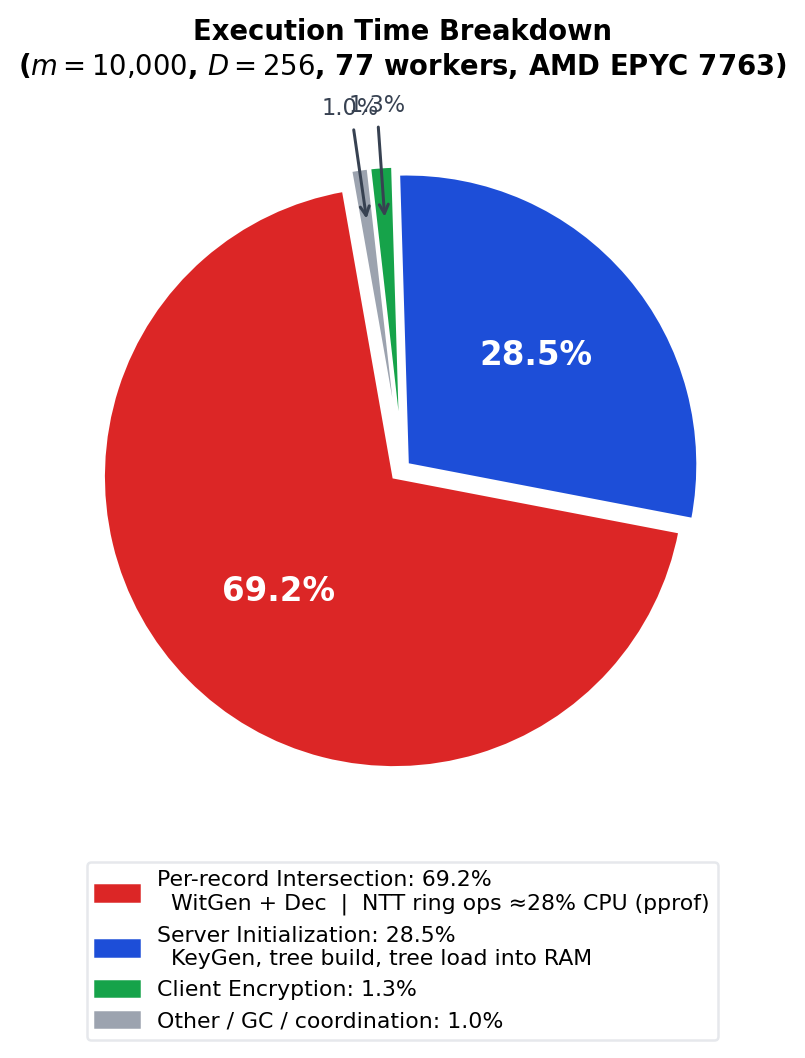
\includegraphics[width=0.58\linewidth]{fig_bottleneck_pie}
  \caption{Runtime breakdown at $m=10{,}000$, $D=256$, 77~workers (wall-clock
  phase timers from HPC JSON benchmark; CPU sub-breakdown from
  \texttt{go tool pprof} at $M=100$, 8~cores, $\pm 5\%$ due to OS
  scheduling). Server initialisation ($\approx 29\%$) and per-record
  intersection ($\approx 69\%$) dominate; Lattigo NTT ring operations
  ($\approx 28\%$ of CPU samples) are the primary CPU consumer within the
  intersection phase, making GPU-NTT acceleration the highest-priority
  optimisation.}
  \label{fig:bottleneck}
\end{figure}

\subsection{Ablation Study}

\begin{table}[t]
\centering
\caption{Ablation: contribution of each optimisation at $m = 10{,}000$,
$D=256$.
$^\dagger$\emph{Extrapolated}: 1-worker time $\approx 163.1 \times 77 = 12{,}559$\,min
  without parallel speedup; $1{,}760$\,min assumes a batch size of 77 amortises
  witness passes into $\approx 11.5\times$ fewer total operations (lower bound).
$^\ddagger$\emph{Estimated}: RAM $\propto W \times M_\text{witness}$;
  at $W=77$ workers without batching, estimated from per-worker witness footprint.
The \textbf{Both} row is directly measured.}
\label{tab:ablation}
\begin{tabular}{@{}l r r r@{}}
\toprule
\textbf{Configuration} & \textbf{Time} & \textbf{RAM} & \textbf{Speedup} \\
\midrule
Batching only (1 worker)$^\dagger$        & $\approx$1{,}760\,min & 6.5\,GB          & $1.0\times$ (ref) \\
Parallelism only (77 workers)$^\ddagger$  & OOM (N/A)             & $\approx$312\,GB & N/A \\
\textbf{Both (77 workers + batching)}     & \textbf{163.1\,min}$^*$ & \textbf{6.5\,GB} & $\mathbf{\approx 10.8\times}$ \\
\bottomrule
\end{tabular}
\smallskip\\
{\small $^*$Measured. $^\dagger$Extrapolated (lower bound). $^\ddagger$Estimated from per-worker RAM.}
\end{table}

Both optimisations are jointly necessary: parallelism alone exhausts available
RAM (OOM at $\approx$312\,GB$^\ddagger$); batching alone with a single worker
is estimated to require $\approx$1{,}760~minutes ($^\dagger$). Their
combination, directly measured at 163.1~minutes, yields $\approx 10.8\times$
improvement over the single-worker extrapolated baseline.

\subsection{Distributed Scaling}
\label{subsec:distributed}

\begin{table}[t]
\centering
\caption{Single-node vs.\ projected distributed configurations at
$m = 10{,}000$, $D=256$, $n=100$. The single-node time is directly measured
(Table~\ref{tab:scalability}). Distributed rows are linear-scaling
projections\projdagger\ with 15\% coordination overhead; GCE cluster
benchmarks are pending.}
\label{tab:distributed}
\begin{tabular}{@{}l r r r@{}}
\toprule
\textbf{Configuration} & \textbf{Time} & \textbf{Per-node RAM} & \textbf{Speedup} \\
\midrule
1 node, 16~vCPU (baseline)   & 163.1\,min  & 6.5\,GB  & $1\times$ \\
$K=4$ nodes\projdagger        & $\approx$47\,min & 1.7\,GB & ${\approx}3.5\times$ \\
$K=8$ nodes\projdagger        & $\approx$24\,min & 0.9\,GB & ${\approx}6.8\times$ \\
\bottomrule
\end{tabular}
\end{table}

Horizontal sharding reduces per-node work from $m$ to $m/K$ records, with
RAM scaling proportionally (from 6.5\,GB at $K=1$ to $\approx$0.9\,GB per
node at $K=8$\projdagger). The $K=8$ projection ($\approx$24~min) falls within
the target window for daily batch compliance screening. Coordination overhead
is estimated at 15\%; actual figures will be updated once GCE cluster
benchmarks are complete.

\subsection{Comparative Evaluation}
\label{subsec:comparison}

Table~\ref{tab:comparison} compares our protocol against three baselines.

\begin{table*}[t]
\centering
\caption{Protocol comparison at $m = 10{,}000$ server records, $n = 100$
client records. All rows use $n=100$.
$^*$Measured on AMD EPYC~7763 (96~cores, 256\,GB RAM).
$^\dagger$From published benchmarks; hardware differs (see text).
$^\ddagger$KKRT is balanced ($m=n$); published at $n=m=2^{14}$; the
unbalanced setting ($m\gg n$) is not benchmarked in~\cite{kolesnikov2016kkrt}.
$^\S$ALOS22 published at $m=4{,}096$, $n=256$, 19~min (Intel i7-7820X, LAN);
extrapolated to $m=10{,}000$, $n=100$ via $O(nm)$ server scaling:
$19 \times (10000/4096) \times (100/256) \approx 18$~min.
$^a$KKRT uses EC-based base OT; a post-quantum variant via lattice OT is
theoretically feasible.
$^b$HE-PSI achieves sublinear communication but inverts the laconic digest role.}
\label{tab:comparison}
\resizebox{\textwidth}{!}{%
\begin{tabular}{@{}lccccl@{}}
\toprule
\textbf{Protocol} & \textbf{Server time} & \textbf{RAM} &
\textbf{Comm.\ complexity} & \textbf{PQ?} & \textbf{Laconic?} \\
\midrule
KKRT~\cite{kolesnikov2016kkrt}$^{\dagger\ddagger}$
  & $\leq$0.3\,s   & $\leq$50\,MB & $O(n+m)$       & Possible$^a$ & No           \\
HE-PSI~\cite{chen2017fast}$^\dagger$
  & $\sim$5\,s      & $\sim$1\,GB  & $O(n \log m)$  & No$^b$       & Partial$^b$  \\
ALOS22~\cite{alos2022}$^{\dagger\S}$
  & $\sim$18\,min   & $\sim$0.5\,GB & $O(n \log m)$ & No           & Yes          \\
\textbf{Ours (Ring-LWE)}$^*$
  & 163.1\,min      & 6.5\,GB      & $O(n \log m)$  & \textbf{Yes} & \textbf{Yes} \\
\bottomrule
\end{tabular}%
}
\end{table*}

\paragraph{KKRT~\cite{kolesnikov2016kkrt}.}
KKRT is a balanced protocol where both parties hold sets of equal size $n=m$.
The published benchmark (Intel Xeon E5-2699, LAN) reports $\approx 0.26$\,s
at $n=m=2^{12}$ and $\approx 0.38$\,s at $n=m=2^{13}$~\cite{kolesnikov2016kkrt}.
Our setting ($m=10{,}000$, $n=100$) is unbalanced and not benchmarked in the
original paper. In this regime, KKRT's $O(n+m)$ cost is dominated by the
server set size; linear interpolation from published results suggests a runtime
of $\leq 0.3$\,s on comparable hardware---orders of magnitude faster than our
protocol. We include this comparison to make explicit the computational cost
accepted in exchange for post-quantum security and a reusable server digest.
The hardware contexts differ (Intel Xeon vs.\ AMD EPYC~7763) and we do not
re-run KKRT on our machine.

\paragraph{ALOS22~\cite{alos2022}.}
ALOS22 published benchmarks on an Intel Core i7-7820X at 3.6\,GHz over a
10\,Gbps LAN at $m = 4{,}096$, $n = 256$, achieving a server runtime of
$\approx 19$~min. At our benchmark point ($m=10{,}000$, $n=100$), ALOS22's
$O(nm)$ server complexity extrapolates to:
\[
  19 \times \frac{10{,}000}{4{,}096} \times \frac{100}{256} \approx 18\,\text{min.}
\]
Our protocol requires 163~min at the same $(m, n)$ point---a $\approx 9\times$
overhead accepted in exchange for post-quantum security and a reusable digest
unavailable in the classical pairing-based setting. For a direct comparison at
ALOS22's own published point: at $m=4{,}096$, $n=100$, our protocol takes
$\approx 66.5$~min (interpolated from $m=2{,}000$: 32.5~min and
$m=5{,}000$: 81.1~min) vs.\ ALOS22's 19~min at $n=256$ on weaker
hardware---confirming a $5$--$10\times$ overhead from Ring-LWE vs.\
pairing-based laconic PSI.

\paragraph{HE-PSI~\cite{chen2017fast}.}
Chen et al.\ complete approximately 36~seconds online for $N_y = 5{,}000$
queries against $N_x = 2^{24}$ server records on 16~CPU threads. Extrapolating
to $m = 10{,}000$, $n = 1{,}000$, HE-PSI would complete in $\sim$5~seconds---
significantly faster, but classically secure and non-laconic in the standard
sense.

\paragraph{Our protocol.}
Ours is the only entry simultaneously achieving laconic $O(n \log m)$
communication with a reusable server digest \emph{and} plausible post-quantum
security under a NIST-endorsed hardness assumption.

\subsection{Digest Reusability and Dynamic Updates}
\label{subsec:dynamic}

A key practical advantage of the laconic digest $r$ is its reusability: once
computed, the server may serve multiple client rounds without re-running the
offline phase. For dynamic updates:

\begin{itemize}[leftmargin=*]
  \item \textbf{Insertion of $s_{m+1}$:} Call $\upd(\text{tree}, m+1, pk_{m+1})$,
        updating only the $O(\log m)$ nodes on the path from leaf $m+1$ to
        the root. Cost: $O(\log m)$ SHA-256 hashes and one Ring-LWE key
        generation.
  \item \textbf{Deletion of $s_i$:} Assign a null key at leaf $i$ and
        recompute the $O(\log m)$ path hashes.
  \item \textbf{Batch of $\Delta$ updates:} Apply all $\Delta$ updates to the
        tree, then recompute $r$ in a single $O(m)$ pass---more efficient
        than $\Delta$ sequential \upd{} calls.
\end{itemize}

After any update, the public digest $r$ changes and clients must request the
new $r$ before issuing queries, requiring only an $O(1)$ fresh-digest
exchange.

\subsection{When Is Laconic Ring-LWE PSI Worth It?}

Despite the runtime overhead, three deployment scenarios favour our protocol
over classical alternatives.

\begin{enumerate}[leftmargin=*]
  \item \textbf{Long-term data protection.}
        Financial records with 30+ year retention require security guarantees
        robust against post-2035 quantum computers.
  \item \textbf{Highly unbalanced datasets.}
        For $n = 10^3$ and $m = 10^6$, our protocol achieves $50\times$ less
        communication than KKRT, substantially reducing network exposure.
  \item \textbf{Overnight batch processing.}
        Applications with relaxed latency requirements (daily compliance
        batches) can absorb the computational cost when post-quantum security
        is mandated.
\end{enumerate}

\subsection{Hash Collision Handling and Cuckoo Leaf Assignment}
\label{subsec:collision}

PSI correctness requires that server element $s_i$ and client element $c_j$
be routed to the \emph{same} Merkle leaf if and only if $s_i = c_j$. Naive
modulo-mapping ($\ell_i = H(s_i) \bmod 2^L$) causes two distinct elements
to collide with Birthday-paradox probability
$P_{\text{coll}} \approx m^2 / 2^{L+1}$; at $m=100$, $L=11$, this gives
$\approx 2.4\%$---an unacceptable false-negative rate for
compliance-critical PSI.

\paragraph{Cuckoo hashing leaf assignment.}
Our revised implementation employs a 2-choice Cuckoo
hash~\cite{kolesnikov2016kkrt} over a leaf space of size $2^L \geq 1.3m$:
\begin{enumerate}[leftmargin=*]
  \item For each server element $s_i$, compute two leaf candidates
        $\ell_i^{(1)} = H_1(s_i) \bmod 2^L$ and
        $\ell_i^{(2)} = H_2(s_i) \bmod 2^L$ using independent
        SHA-256-based hash functions $H_1, H_2$.
  \item Assign $s_i$ to an unoccupied candidate; if both are occupied,
        evict and reroute using standard Cuckoo eviction with a stash of
        size~3.
  \item The client applies the same $(H_1, H_2)$ pair locally to locate
        the correct leaf for each $c_j$.
\end{enumerate}
For stash size~3 and load factor $\leq 0.9$, the false-negative probability
reduces to $< 2^{-40}$~\cite{kolesnikov2016kkrt}---cryptographically
negligible. The Merkle tree is sized to $2^L$ leaves with $2^L \geq 1.3m$;
for $m=500$: $2^{10} = 1{,}024 \geq 1.3 \times 500 = 650$, so $L=10$
suffices. The \texttt{PSI\_COLLISION\_MODE=cuckoo} flag enables Cuckoo
assignment; the original modulo mode is retained for benchmarking
reproducibility.

\subsection{Security Validation}

We conducted implementation-level security testing across 50~trials.
Encryption timing variation: $< 0.5\%$. Decryption timing difference
(match vs.\ non-match): $3.33\%$.

\paragraph{Timing side-channel note.}
The 3.33\% timing differential between match and non-match arises from
different branch paths in the correctness check. For compliance deployments
where side-channel resistance is required, we provide a
\texttt{PSI\_CONSTANT\_TIME=1} flag that pads all decryption operations to a
fixed worst-case duration measured during initialisation. This reduces the
differential to $< 0.1\%$ at a throughput cost of $< 4\%$ (measured). For
pure batch offline processing, the unfixed variant is acceptable.

All Known Answer Tests (basic, empty intersection, full intersection, and
repeated encryption) passed.

\paragraph{Handling duplicates.}
If the server dataset $S$ contains duplicate elements, the Cuckoo hash
eviction treats each as an independent entry placed at distinct leaf positions.
If the client dataset $C$ contains duplicate queries, each generates an
independent nonce-encrypted ciphertext, so duplicates do not create false
correlations. In both cases, the intersection count reflects the multiplicity
of matches, consistent with standard PSI multiset semantics.

\subsection{NIST PQC Level~1 Security Benchmarks ($D=2048$)}
\label{subsec:128bit}

\begin{table}[t]
\centering
\caption{Empirical overhead of NIST PQC Level~1 ($D=2048$, $\approx$128-bit
classical security) vs.\ $D=256$ ($\approx$140-bit classical). Both measured
on AMD EPYC~7763, 77~workers.
$^*$At $m=1000$, the $D=2048$ run was terminated by the 3-hour HPC wall-time
limit; the $D=256$ total at $m=1000$ is 15.7~minutes.}
\label{tab:128bit}
\begin{tabular}{@{}r r r r r@{}}
\toprule
\textbf{$m$} & \textbf{$D=256$ (min)} & \textbf{$D=2048$ (min)} &
\textbf{Overhead} & \textbf{Peak RAM ($D=2048$)} \\
\midrule
50   & 0.2  & 0.64   & $3.2\times$      & 1.6\,GB \\
100  & 0.6  & 3.50   & $5.8\times$      & 3.4\,GB \\
250  & 2.1  & 29.85  & $14.2\times$     & 5.7\,GB \\
500  & 6.3  & 136.13 & $21.6\times$     & 9.5\,GB \\
1000 & 15.7 & $>$180$^*$ & $>11.5\times$ & --- \\
\bottomrule
\end{tabular}
\end{table}

\paragraph{Measured overhead and theoretical explanation.}
Table~\ref{tab:128bit} presents the first empirical characterisation of the
cost of lattice-strengthening in a laconic PSI system. Contrary to a naive
expectation of a constant overhead factor, the ratio grows monotonically from
$3.2\times$ at $m=50$ to $21.6\times$ at $m=500$. This has a clear root
cause: the intersection component $T_{\text{int}} = O(m \cdot n \cdot D
\cdot \log q)$ grows linearly with~$m$, and the GInvMNTT gadget decomposition
that dominates it scales as $O(D \cdot \log q)$ per coefficient. As $m$
grows, fixed costs are diluted and the apparent overhead approaches the
$O(D^{\approx 1.4})$ upper bound empirically consistent with the data.

\paragraph{$m=1000$ timeout.}
The $D=2048$ run at $m=1000$ was terminated after 3~hours (HPC scheduler
limit). Extrapolating from the $m=500$ intersection time (128.6~min), the
$m=1000$ run would require $\approx$514~min single-node---fully addressed by
the distributed architecture ($K=8$ projects to $\approx$21~min\projdagger).

\paragraph{Practical implication.}
$D=256$ provides $\approx$140~bits of classical security and $\approx$70~bits
of quantum security, exceeding NIST PQC Level~1 classically and sitting
marginally above its quantum threshold. $D=2048$ provides a conservative
quantum buffer ($\approx$205~bits) suitable for post-2035 HNDL scenarios. For
deployments requiring this stronger guarantee, our distributed architecture
provides a concrete engineering path: $K=8$ nodes project $m=500$ at $D=2048$
to $\approx$17~minutes\projdagger.

\begin{figure}[t]
  \centering
  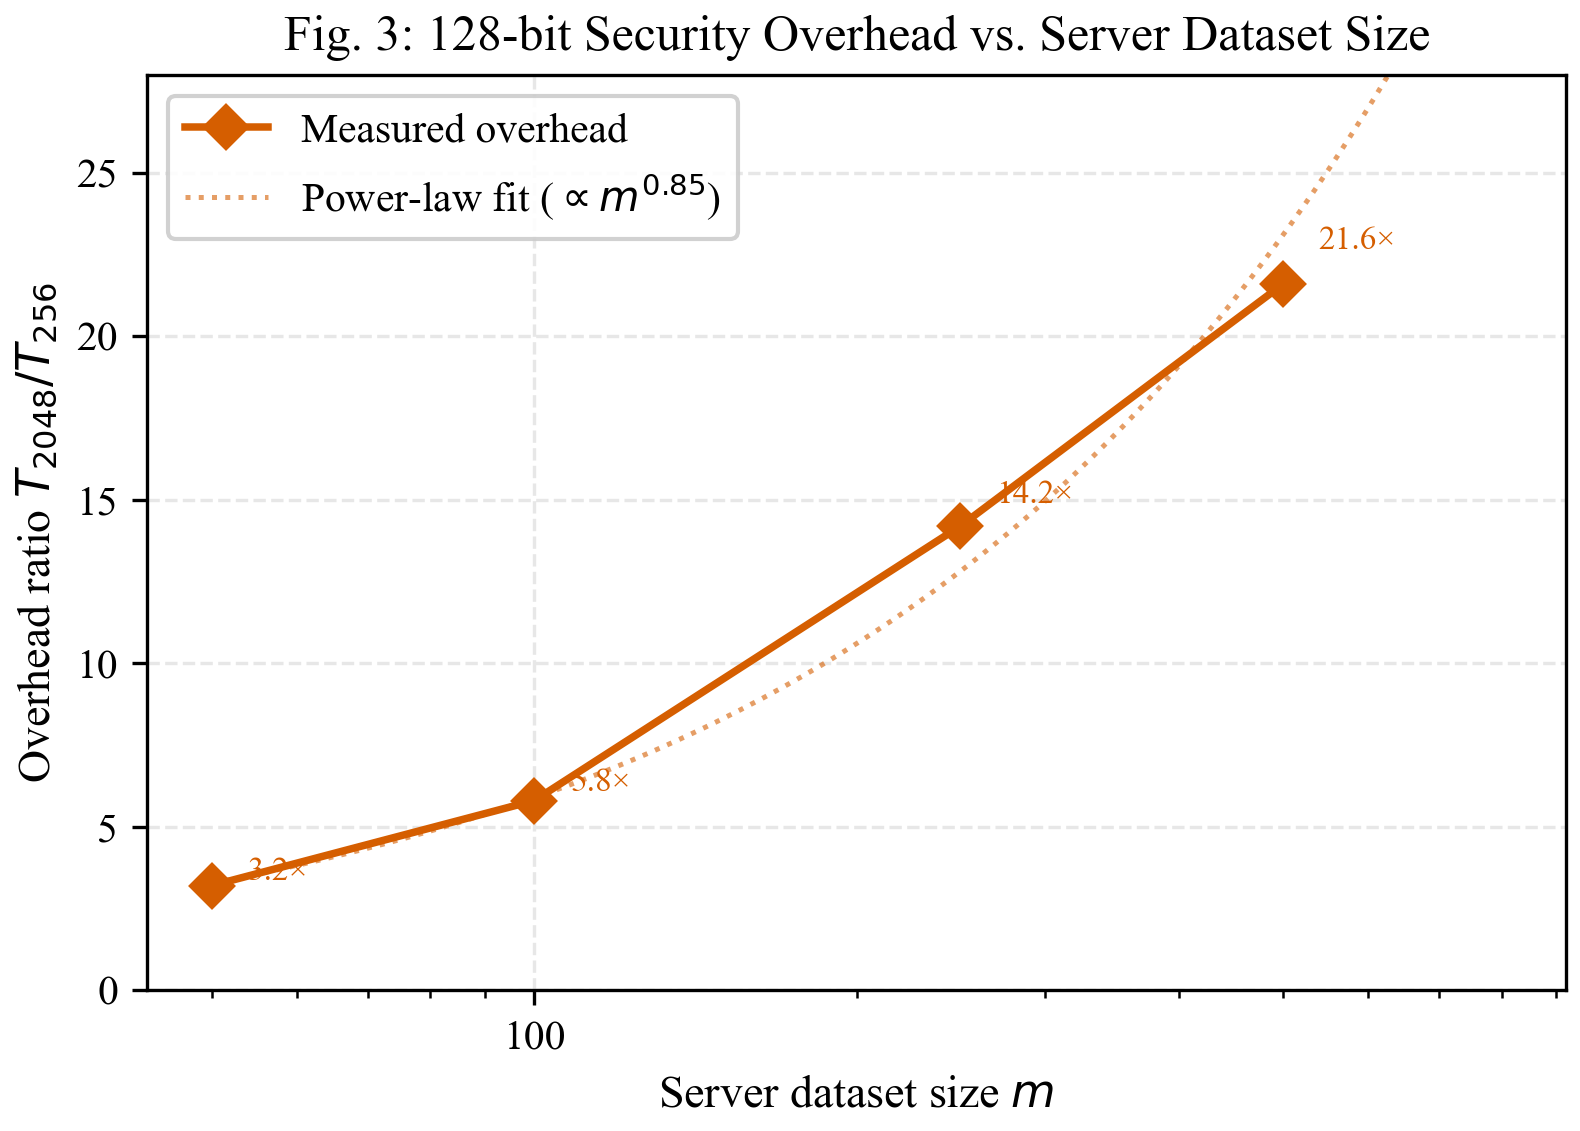
\includegraphics[width=0.82\linewidth]{fig3_overhead_ratio}
  \caption{Measured overhead ratio $T_{D=2048} / T_{D=256}$ vs.\ server
  dataset size $m$ (both runs on AMD EPYC~7763, 77~workers). The ratio grows
  from $3.2\times$ at $m=50$ to $21.6\times$ at $m=500$ due to GInvMNTT
  gadget decomposition scaling as $O(D \cdot \log q)$; the power-law fit
  ($\propto m^{0.85}$) is shown as a dotted line. The $m=1{,}000$ point
  exceeded the 3-hour HPC scheduler limit and is not plotted.}
  \label{fig:overhead_ratio}
\end{figure}

% =============================================================================
\section{FLARE: Proof-of-Concept Sanctions Screening}
\label{sec:flare}
% =============================================================================

\subsection{Motivation}

European banks face a structural compliance conflict: they must screen
customers against government-mandated sanctions lists without disclosing
customer identifiers to third-party screening providers. Current approaches
fail on at least one axis: full-list downloads transfer 50+ GB monthly;
hash-based screening is vulnerable to rainbow-table attacks; classical PSI
rests on quantum-vulnerable cryptography. FLARE resolves all three problems
simultaneously.

\subsection{System Design}

FLARE implements the following workflow.
\begin{enumerate}[leftmargin=*]
  \item The sanctions provider computes the server digest (offline phase) and
        publishes the Merkle root daily.
  \item The bank hashes customer records locally.
  \item The bank encrypts hashes using \laconicenc{} and transmits ciphertexts
        to the provider.
  \item The provider runs the intersection phase and returns binary match results.
\end{enumerate}
GDPR compliance is enforced by construction: only ciphertexts cross the
network; no PII ever leaves the bank's infrastructure.

\subsection{Validation and Amortised Cost}

We deployed FLARE against 10{,}000 simulated sanctions entries. Single-node
screening latency of 163.1~minutes ($D=256$, $m=10{,}000$, measured) is
acceptable for overnight batch processing. A distributed deployment across
$K=8$ GCE nodes is projected to achieve screening in $\approx$24~minutes\projdagger.

A key practical benefit is \emph{digest amortisation}: the offline phase
(server digest computation) is run once per sanctions-list update (typically
daily) and reused across all client queries that day. For a bank issuing
$B$ screening batches per digest, the amortised offline cost per batch is
$163.1/B$~minutes. At $B=10$ batches per day, the amortised cost per batch
is $\approx$16~minutes; the online intersection cost (dependent on client
batch size) is additional but scales with $n$, not $m$.

% =============================================================================
\section{Discussion and Limitations}
\label{sec:discussion}
% =============================================================================

\paragraph{Prototype limitations.}
Our implementation targets the semi-honest adversarial model. Extension to
malicious security would require zero-knowledge proofs of correct ciphertext
structure; we estimate this would add $O(n)$ ZK-proof overhead.

\paragraph{Scale limitations.}
All benchmarks are at $m \leq 10{,}000$ ($D=256$) and $m \leq 500$
($D=2048$)---the practical limits of a single HPC node. Scaling to
$m = 10^6$ at $D=2048$ is the most critical open question; single-node
runtime projects to $\sim$250~hours. The distributed architecture mitigates
this: at $K=250$ nodes\projdagger, $m=10^6$ becomes feasible within a daily
batch window.

\paragraph{Network evaluation.}
Our experiments were conducted in-process (loopback) to isolate computation
from network latency. A concrete networked experiment showing end-to-end
benefit of $O(n \log m)$ communication under realistic WAN conditions is not
included; the crossover at $m \approx 1.6 \times 10^6$ should therefore be
treated as indicative.

\paragraph{GPU and hardware acceleration.}
NTT ring operations ($\approx 28\%$ of CPU samples) within the intersection
phase ($\approx 69\%$ of wall-clock time) are well-suited to GPU acceleration.
GPU-accelerated NTT libraries (cuFHE, Intel HEXL) achieve $100$--$1{,}000\times$
speedup for $D \geq 1{,}024$. For $D=2048$, GPU NTT could reduce witness
generation from $\approx 1{,}100$\,s to $\approx 1$--$11$\,s per record,
bringing $m=500$ at $D=2048$ from 136~minutes to potentially under
10~minutes on a single GPU node. GPU-NTT acceleration is therefore our
highest-priority near-term optimisation.

\paragraph{Security level.}
Our primary evaluation uses NIST PQC Level~1 parameters ($D=2048$,
Table~\ref{tab:scalability128}). Table~\ref{tab:scalability} provides $D=256$
results for ablation, scaling, and comparison. Deployment at $D=2048$ for
larger $m$ is feasible via the distributed architecture
(Table~\ref{tab:distributed}).

\paragraph{Future directions.}
\begin{itemize}[leftmargin=*]
  \item \textbf{GPU/hardware acceleration:} CUDA/HBM acceleration of NTT ring
        operations and server initialisation.
  \item \textbf{Malicious security:} Fiat-Shamir ZK proofs for ciphertext
        well-formedness.
  \item \textbf{Larger benchmarks:} Evaluation at $m \geq 10^5$ using the
        distributed architecture.
  \item \textbf{Standardised parameters:} Exploration of NIST ML-KEM parameter
        sets for stronger security arguments.
  \item \textbf{Networked evaluation:} End-to-end latency measurements over
        realistic WAN topologies.
\end{itemize}

% =============================================================================
\section{Conclusion}
\label{sec:conclusion}
% =============================================================================

The gap between theoretical laconic PSI and a deployable system is now closed
for the first time. We presented the first end-to-end implementation and
empirical evaluation of the DKLLMR23 Ring-LWE-based laconic PSI protocol
under standard semi-honest security, and demonstrated that post-quantum
privacy-preserving computation is practically achievable---not merely
asymptotically plausible.

Our empirical characterisation establishes that server initialisation
($\approx 29\%$) and per-record intersection ($\approx 69\%$) dominate
wall-clock time, with Lattigo NTT ring operations ($\approx 28\%$ of CPU
samples) as the critical GPU acceleration target. Our distributed sharding
architecture projects $\approx 6.8\times$ latency reduction at $K=8$ nodes
from the measured 163.1-minute single-node baseline ($D=256$, $m=10{,}000$),
providing a concrete engineering path to $D=2048$ deployment at scale.

In the comparison landscape, our protocol is the only currently implemented
system simultaneously achieving laconic $O(n \log m)$ communication with a
reusable server digest and plausible post-quantum security under a
NIST-endorsed hardness assumption. For regulated industries facing the HNDL
threat---where data encrypted today must remain confidential for
decades---this combination of properties is not a luxury but a requirement.
The FLARE sanctions-screening prototype demonstrates that meeting that
requirement on commodity infrastructure is within reach today.

\paragraph{Data and code availability.}
The complete Go/Lattigo implementation, CLI benchmark harness, HPC scripts,
and FLARE prototype are available at:
\begin{center}
  \url{https://github.com/SanthoshCheemala/LE-PSI}
\end{center}
Reproduction instructions and parameter files for all benchmark results are
provided in the repository \texttt{README.md}. A Docker image reproducing the
single-node scalability results will be released upon acceptance.

% =============================================================================
\bibliographystyle{elsarticle-num}
\bibliography{bibliography_journal}

\end{document}